\chapter{Preliminary Research}\label{research}\label{section \thechapter}

\mySection{Sand-drawing robots}{\SW}\label{sand-drawing robots}
    \begin{wrapfigure}{I}{0.45\textwidth}
      \begin{center}
        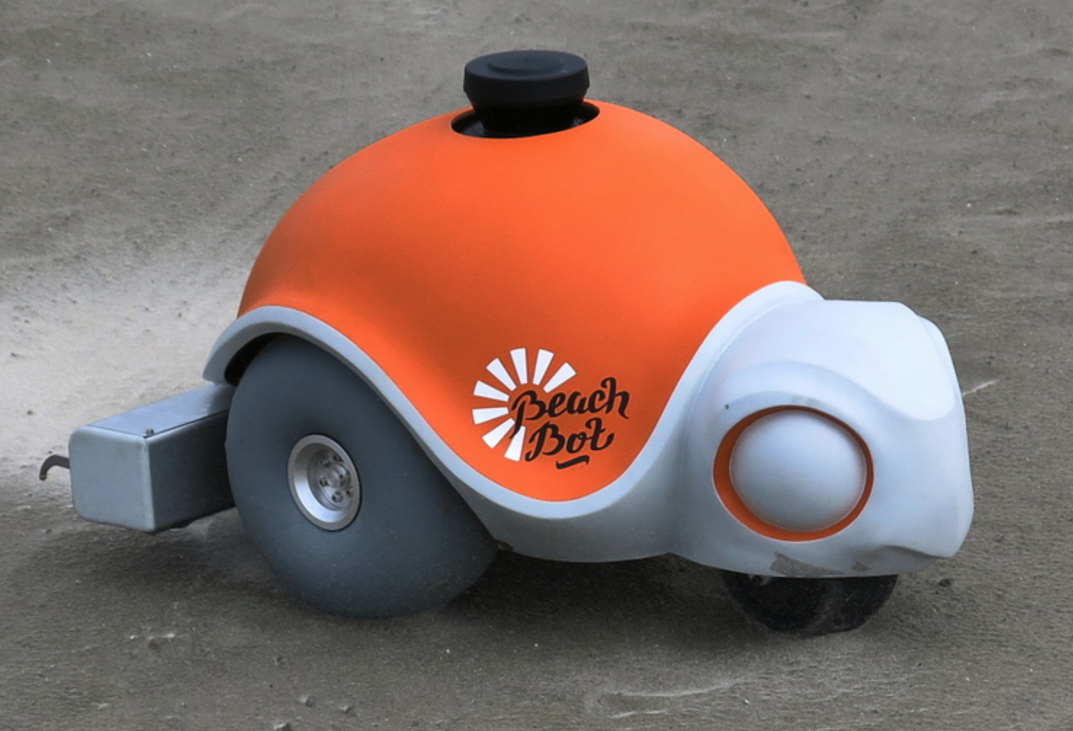
\includegraphics[width=0.43\textwidth]{Files/beachbot}
      \end{center}
      \caption{ETH Z{\"u}rich's BeachBot robot.{\small (Retrieved from \citen{beachbot} on 2016--01--28)}}
      \label{fig: beachbot}
    \end{wrapfigure}
    The `best-in-class', and indeed only notable, beach-scale drawing robot is Disney's BeachBot (Figure~\ref{fig: beachbot}), produced by ETH Z{\"u}rich.\cite{beachbot} The robot is capable of drawing images in the sand -- this has particular application in marketing Disney's sea themed--franchises and providing entertainment at Disney's beach resorts.\\
    The robot's drawing mechanism consists of fourteen rake teeth mounted in pairs on seven servo motors -- this allows lines of varying width (or no lines) to be drawn. The BeachBot is driven by two rear wheels and steered by a front wheel -- in a three-wheel configuration. It is fairly compact, measuring only sixty centimeters in length. BeachBot's chassis is enclosed in a sealed aluminum shell to protect its components from the sand. From this shell a laser scanner (part of BeachBot's guidance system) protrudes. The laser scanning guidance system directs BeachBot to draw its programmed image relative to reflecting posts installed by the user; this provides a `canvas' on which BeachBot works.\\
    BeachBot's shell is design to give it the appearance of a  turtle from Disney's \emph{Finding Nemo} property -- not only does this incorporate Disney's brand image into the design, but it also provides a non-threatening look. The latter point will be important for our robot since it will need to operate on a beach, an environment in which people are not used to seeing machinery.\\
    It has been suggested that with modification BeachBot could be used on snowy terrain to promote Disney's winter themed--franchises.

    \begin{wrapfigure}{O}{0.45\textwidth}
      \begin{center}
        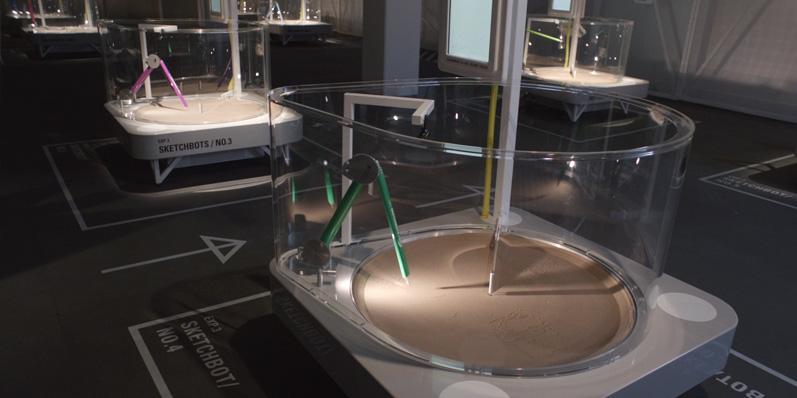
\includegraphics[width=0.43\textwidth]{Files/sketchbots}
      \end{center}
      \caption{Google Chrome Web Lab's sketchbots at the Science Museum, London.{\small (Retrieved from \citen{chromeweblab} on 2016--02--02)}}
      \label{fig: sketchbots}
    \end{wrapfigure}
    Although not beach-scale, Google has produced tabletop-scale sand art machines called `sketchbots' (Figure~\ref{fig: sketchbots}) (Operational at the Science Museum in London between 2012 and 2013).\cite{Warman2012} The robot itself was integrated with the tabletop; it comprised an arm with a mounted stylus and a `sweeping' implement, which moved in a circular motion, to clean the sand canvas. The robot took an input of the user's face from a camera, parsed the image and then drew it in the sand. Google  created the installation as part of its `Chrome Web Lab', showcasing modern web technologies such as HTML5.

\mySection{Movement}{\SW}
    In considering the robot's locomotion, the terrain over which it will travel (sand -- potentially damp) and its purpose (drawing) are center-stage. The robot must have sufficient traction to travel over a beach. When considering the requirement that it draw, it must be able to turn as tightly as instructed to avoid incongruity between programmed and drawn images. It may also be possible to incorporate any turning limitations into the child's programming interface, such that an impossible turn cannot be instructed. It would also be far from ideal for the robot to obscure any lines it had already drawn when pathing back over them.

    The main methods of robot locomotion that might be relevant are wheeled (or caterpillar tracked), walking, rolling, or slithering. Considering the scope of this project, and the budget available, the latter options are not viable. Companies such as Boston Dynamics have budgets of millions of dollars to work on the development of walking technology -- achieving a robot capable of walking is a significant feat, even before considering drawing. While rolling or slithering may potentially be workable, they would contribute significant design complications to any kind of `on/off' functionality. Flying private drones have increased in popularity dramatically; in considering a drone type robot as an option, the main challenges are the extreme comparative difficulty of achieving flight compared with traction and drawing a line in the sand. Creating a flying drone from scratch would pose many challenges, which it is unlikely we could surmount with this project's resources. The marker design also poses significant challenges -- a marker fixed rigidly to a drone is likely to interfere with flight and a free-hanging marker runs the risk of not providing enough pressure to create a line. The most viable locomotion solutions are caterpillar tracks and wheels.\\
    Caterpillar tracks combine very capable terrain handling with on-a-point turning, however they are very likely to disrupt the line left behind the robot, especially when on-a-point turning.  With the right design and material, wheels might prove sufficiently able to handle the terrain and also cause limited harm to the robot's drawn lines. Such wheels would need to have a large surface area and be made of a reasonably soft material (\eg soft touch plastic) -- minimizing the robot's overall weight would also be important in making such a design choice viable. Although wheels open opportunities in terrain handling and line preservation, they come up short of caterpillar tracks on turning ability. A short wheelbase might go some way to improve this. There is also the potential of a three-wheel configuration, instead of four (or more) wheels -- this was implemented in Disney's BeachBot (Section~\ref{sand-drawing robots}) to the benefit of the robot’s turning circle. It should be noted that a three-wheel design raises stability concerns. Ultimately the decision between caterpillar tracks and wheels comes to a question of whether, or to what extent, the child instructing the robot should be limited in their design.

\mySection{Digging mechanisms}{\SW}
    At its most basic level, a beach-scale sand drawing robot need only leave a line in the sand wherever it travels, in order to produce a picture -- this poses a severe constraint on what can be drawn. In the case of our educational robot, the child would have the limitation of instructing the robot to draw a picture with only a single continuous movement. This `always on' approach to the drawing mechanism can be improved upon.

    Instead of fixing the robot's marking implement, it could be built to raise or lower, adding `on/off' drawing functionality. The marking implement, or `marker', could be fitted to an actuator to achieve this. The actuator could be linear or rotary; a linear actuator would lend itself to a marker below the robot chassis, while a rotary actuator would be more appropriate for a marker behind the chassis, like a rake tooth (as is being used in Figure~\ref{fig: andres amador}). A rear mounted, rake-like design might provide a more fluid, pulling movement through the sand. There are precedents for this positioning choice: Disney's BeachBot (Section~\ref{sand-drawing robots}) and plough attachments for tractors. While the addition of an actuator significantly improves the robot's drawing flexibility, it would be vulnerable to sand in its mechanism and would add cost, should one not be salvageable from spare parts. The use of an actuator would also place a small requirement on the robot's power supply.\\
    The marker itself needs to exert sufficient force on the sand to leave a line behind the robot, without acting as a brake -- this would inhibit the robot's movement. Inhibition of the robot's movement would lead to significant deviation in the drawn image compared to the programmed image. The key to avoiding this is to create a marker with appropriate depth; the marker should not penetrate so deep in the sand as to invite significant resistance to its motion, while reaching deep enough to leave a sufficient (\emph{i.e.} visible) line.\\
    Implementing software to vary the depth of the marker could serve to mitigate any issues arising from resistance, and also could ensure trouble does not arise on uneven beach area. The limitations here lie within the realm of software development, and potentially the requirement that the actuator provide feedback.\\
    Within these parameters the marker itself could be varied -- for instance having multiple markers would provide a different pattern to the line. These multiple markers could be fitted to more actuators (with the potential of substantially increased cost) to allow for a variable line width.

    An alternative marker approach would be that of a cylindrical `drum'. Such a cylinder could have a pattern embossed upon it that would leave a pattern as the robot's marking. Gunilla Klingberg's `sand machine' (Section~\ref{art review}, Figure~\ref{fig: sand machine}) uses this approach. This approach could be implemented with `on/off' functionality, but would allow for only a preset pattern in the line. The implementation of a patterned line of varying width (\eg multiple drums with raising and lowering ability) could prove very problematic. Such an implementation of this method would be best achieved in a manner similar to NASA's RASSOR digging robot -- a drum separate from the locomotion mechanism that can be lowered and raised.\cite{Siceloff2013} In a similar way, the NASA's Curiosity rover leaves the pattern for ``JPL'' in Morse code in its tracks as it travels across the Martian surface.

\mySection{Construction materials}{\AK}
    An important consideration when deciding on a material for the body and base of the robot is the penetration into the sand. A denser material will cause the robot to sink more, but lighter materials will mean a compromise in strength, stability, or price. However, if the wheels or tracks of the robot are wise enough, there may be some freedom when deciding what materials the components of the robot should be made of.\\
    Researchers at the Georgia Institute of Technology have been able to vary the strength of the supporting ground by using varying air flow from beneath.\cite{Qian} This has allowed them to vary the stiffness of the sand and observe the performance of a robot on these surfaces.

    The robot should be made to be water resistant; contact with water at some point is inevitable and water coming into contact with the electrics would reduce the lifespan and reliability of the machine. Damage caused by sand should also be a consideration: the machine is likely to come into contact with a substantial amount of sand. Sand is silica, which is very abrasive; if this abrasion occurs around the more sensitive areas of the machine it could cause extensive damage. Sandusa is a range of beach products that are water- and sand-proof.\cite{sandusa} This is due to a smooth nylon material that allows sand to slide off easily combined with an inner waterproof lining. This material could be used to protect the robot.
